%\documentclass{standalone}
%\usepackage{tikz}
%\usepackage{pgfplots}

%\begin{document}
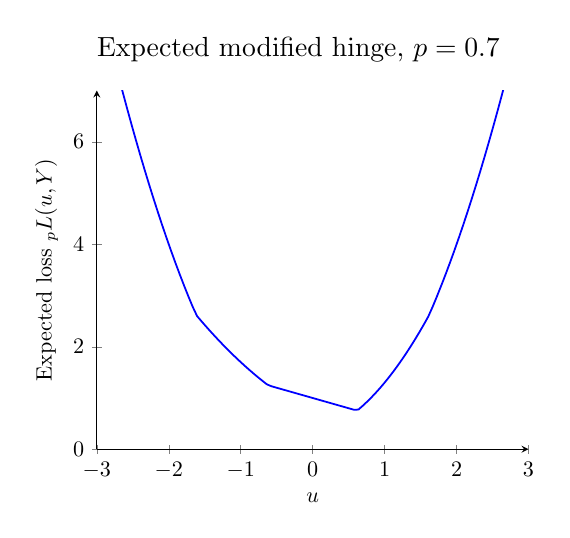
\begin{tikzpicture}[scale=0.8, thick]
    \begin{axis}[
        axis lines = left,
        xlabel = $u$,
        ylabel = {Expected loss $\E_{p} L(u,Y)$},
        xmin = -3,
        xmax = 3,
        ymin = 0,
        ymax = 7,
        grid = none,
    ]
    % Plot the function
    \addplot[
        domain=-3:3,
        samples=100,
        color=blue,
        thick
    ]
    {0.7 * max(x * x, 1 - x) + 0.3 * max(x * x, 1 + x)};
    \end{axis}
    \node[above] at (3.2, 6){Expected modified hinge, $p = 0.7$};
\end{tikzpicture}
%\end{document}
